\documentclass[a4paper, 12pt]{article}

\usepackage{enumerate}
\usepackage{hyperref}
\hypersetup{
	colorlinks=true,
	linkcolor=blue,
	filecolor=blue,
	urlcolor=blue,
	citecolor=blue,
}
\usepackage{amsmath}
\usepackage{amsthm}
\usepackage{amssymb}
\usepackage[margin=3cm]{geometry}
\usepackage{mathpazo}
\usepackage{url}
\usepackage{subcaption}
\usepackage{tikz}
\usepackage{pgf}
\usepackage{longtable}
\usepackage{multirow}
\usepackage{graphicx}
\usepackage{pgfplots}
\usepackage{cleveref}
\usepackage{amsrefs}
\usepackage{bbm}
\usepackage{csquotes}
\usepackage{wrapfig}
\usepackage{algorithm}
\usepackage{algpseudocode}
\usepackage{mathrsfs}
\usepackage{afterpage}

\numberwithin{equation}{section}
\numberwithin{figure}{section}

\newtheorem{thm}{Theorem}[section]
\newtheorem*{thm*}{Theorem}
\newtheorem*{con*}{Conjecture}
\newtheorem{lem}[thm]{Lemma}
\newtheorem{prop}[thm]{Proposition}
\newtheorem{cor}[thm]{Corollary}
\newtheorem{lemma}[thm]{Lemma}
\newtheorem{conj}[thm]{Conjecture}

\theoremstyle{definition}
\newtheorem{defn}[thm]{Definition}
\newtheorem{remark}[thm]{Remark}
\newtheorem{ex}[thm]{Example}
\newtheorem{quest}[thm]{Question}
\newtheorem{obs}[thm]{Observation}

\renewcommand{\leq}{\leqslant}
\renewcommand{\geq}{\geqslant}
\newcommand{\N}{\mathbb{N}}
\newcommand{\Z}{\mathbb{Z}}
\newcommand{\Q}{\mathbb{Q}}
\newcommand{\R}{\mathbb{R}}
\newcommand{\C}{\mathbb{C}}
\newcommand{\tr}{\mathrm{t}}
\newcommand{\WEEK}[1]{%
\hfill Week #1

\vspace{-1em}

\begin{center}
	\rule{\textwidth}{2pt}
\end{center}
\vspace{0.5em}%
}

\renewcommand{\algorithmicrequire}{\textbf{Input:}}
\renewcommand{\algorithmicensure}{\textbf{Output:}}

\setcounter{tocdepth}{2}

\allowdisplaybreaks

\title{Geometric Foundations of Data Analysis I: \\ Week 3}
\author{Joshua Maglione}
\date{22 September 2025}

\begin{document}

\maketitle
\tableofcontents

\setcounter{section}{2}
\setcounter{subsection}{7}
\setcounter{thm}{1}

\subsection{Nonlinear fittings}\label{sec:nonlinear-fittings}

Although all of our examples so far have been linear fittings, we will
demonstrate that least squares fittings works in the nonlinear case. What is
important is that we have a candidate equation to fit. In the linear cases, we
tried to fit 
\[ 
	y = b_0 + b_1x_1 + b_2x_2 + \cdots + b_{p-1}x_{p-1}.
\] 

Suppose we have the following data as given in \Cref{fig:nonlinear-data}.
Instead of trying to fit the line $y=b_0+b_1x$, we could try to fit the
parabola: 
\[ 
	y = b_0 + b_1x + b_2x^2. 
\] 
We can treat this the same way as before. Of course the quantities $x$ and $x^2$ are \textit{not} independent, but we can ignore this. Set 
\begin{align*} 
	x_{i1} &= x_i, & x_{i2} &= x_i^2.
\end{align*} 
Therefore, the hyperplane of best fit for the data $(x_{i1}, x_{i2}, y_i)$ will
give us the parabola of best fit. \textit{Try this on your own!} 

\begin{figure}[h]
	\centering
	\begin{minipage}{0.3\textwidth}
		\centering
		\begin{tabular}{cc}
			$x_i$ & $y_i$ \\ \hline
			2.27 & 2.50 \\
			5.06 & -16.13 \\ 
			1.45 & 4.23 \\ 
			5.89 & -22.46 \\
			0.48 & 1.37 \\ 
			-0.22 & 0.86 \\ 
			1.44 & 11.85 \\ 
			-1.77 & -14.71 \\ 
			2.45 & 9.42 \\ 
			-1.54 & -14.07 \\ 
			7.55 & -55.62 \\ 
			1.76 & 4.45 \\ 
			5.16 & -19.56 \\ 
			3.26 & -2.79 \\
			3.23 & 5.20 \\
			0.85 & 8.09
		\end{tabular}
	\end{minipage}~%
	\begin{minipage}{0.65\textwidth}
		\centering
		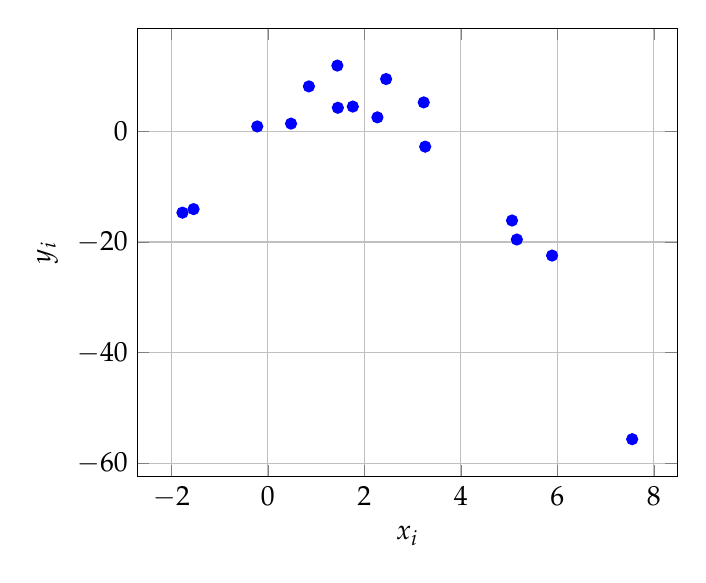
\begin{tikzpicture}
			\begin{axis}[
				xlabel=$x_i$,
				ylabel=$y_i$,
				grid=both,
			]
			\addplot[only marks, mark=*, mark size=2pt, color=blue] coordinates {
				(2.27, 2.50)
				(5.06, -16.13)
				(1.45, 4.23)
				(5.89, -22.46)
				(0.48, 1.37)
				(-0.22, 0.86)
				(1.44, 11.85)
				(-1.77, -14.71)
				(2.45, 9.42)
				(-1.54, -14.07)
				(7.55, -55.62)
				(1.76, 4.45)
				(5.16, -19.56)
				(3.26, -2.79)
				(3.23, 5.20)
				(0.85, 8.09)
			};
			\end{axis}
		\end{tikzpicture}
	\end{minipage}
	\caption{Data points demonstrating a nonlinear relationship.}
	\label{fig:nonlinear-data}
\end{figure}

So one can fit any hypersurface $y=f(x_1,\dots, x_{p-1})$ to the given data. The
function $f$ in this case is called the \textbf{regression function}. This
general method of analysis is known as \textbf{regression analysis}. A few
questions arise:
\begin{itemize}
	\item Which surface is ``best''?
	\item How can we quantify ``best''?
	\item Even in the line case $(p=2)$, how can we quantify how well data fits
	our line? 
\end{itemize}

\subsection{Coefficient of determination ($R^2$ values)}

We are going to make precise how well our hyperplane fits our data. Recall that
hyperplanes can be replaced by hypersurfaces; see \Cref{sec:nonlinear-fittings}.
First we establish some notation. Suppose we have $n$ data points $(x_{i1},
x_{i2}, \dots, x_{i,p-1}, y_i)\in \R^p$. Then we define  
\begin{align*}
	\text{(Fitted value)} & & \widehat{y}_i &= b_0 + b_1x_{i1} + b_2 x_{i2} + \cdots + b_{p-1} x_{i,p-1}, \\
	\text{(Residual)} & & e_i &= y_i - \widehat{y}_i, \\
	\text{(Sample mean)} & & \overline{y} &= \frac{1}{n}\sum_{i=1}^n y_i.
\end{align*}
These yield vectors in $\R^n$ as follows 
\begin{align*}
	\widehat{Y} &= \begin{pmatrix}
		\widehat{y}_1 \\ \vdots \\ \widehat{y}_n
	\end{pmatrix} = XB, & 
	E &= \begin{pmatrix}
		e_1 \\ \vdots \\ e_n
	\end{pmatrix} = Y - \widehat{Y}, & 
	\overline{Y} &= \begin{pmatrix}
		\overline{y} \\ \vdots \\ \overline{y}
	\end{pmatrix} = \overline{y} \begin{pmatrix}
		1 \\ \vdots \\ 1 
	\end{pmatrix}. 
\end{align*}

From our $n$ data points, we have three points in $\R^n$ given by $Y$,
$\widehat{Y}$, and $\overline{Y}$. Three points always lie on a plane, so the
three point determine a triangle on such a plane. What does this triangle look
like? If it is a triangle (and not a line or a single point), then the next
lemma proves it must be a right triangle.

\begin{lem}\label{lem:orthog}
	The vectors $E = Y - \widehat{Y}$ and $\widehat{Y}-\overline{Y}$ are
	orthogonal.
\end{lem}

\begin{proof}
	Suppose $X^{\tr}XB = X^{\tr}Y$. We need to prove two equations. For the
	first, 
	\begin{align*}
		0 &= X^{\tr}(Y - XB) = X^{\tr}(Y - \widehat{Y}) = X^{\tr}E.
	\end{align*}
	Hence, $X^{\tr}E=0$. For the second, 
	\begin{align*}
		\overline{Y}^{\tr}E &= \overline{y} \sum_{i=1}^n (y_i - \widehat{y}_i) \\
		&= \overline{y} \sum_{i=1}^n (y_i - (b_0+b_1x_{i1} + b_2x_{i2} + \cdots + b_{p-1}x_{i,p-1})) \\
		&= -\dfrac{\overline{y}}{2} \cdot \dfrac{\partial S}{\partial b_0} = 0,
	\end{align*}
	where $S$ is defined in the Week 1 Notes, so $\overline{Y}^{\tr}E=0$.
	Thus, we have 
	\begin{align*}
		(\widehat{Y} - \overline{Y}) \cdot E &= (XB)^{\tr} E - \overline{Y}^{\tr}E = 0. \qedhere
	\end{align*}
\end{proof}

\begin{remark}
	One can simplify the proof for Lemma~\ref{lem:orthog} by applying an isometry to
	the data, so that $\overline{y} = 0$. That is, one only needs to prove that
	$E$ and $\widehat{Y}$ are orthogonal.
\end{remark}





























\end{document}